\section{Neural Network}
\label{sec:NN}
In this article, we focus mainly on supervised learning rather 
than unsupervised learning. In most cases, the tasks of neural 
networks turn out to be regression, binary classification for 
instance. Generally speaking, a neural network approximate a
function by minimizing the difference between the ideal one and
the approximated one. In short, what neural networks do is optimization.
\par In this section, we start with the representation of a neural
network and then further into the way neural networks solve an
optimization problem.

\subsection{Neuron}
Neuron is an abstract representation of the smallest component of
a neural network. Specifically neuron is a type of function 
$ g: \mathbb{R}^n \rightarrow \mathbb{R}^n $, which is also called 
activation function including ReLU, sigmoid, softmax etc. In various 
neural networks such as Deep Neural Network, Convolution Neural 
Network (CNN) and Recurrent Neural Network (RNN), neuron takes on 
difference forms.
\par The basic model of neuron is illustrated in \autoref{fig:neuron}.
We denote that $ x \in \mathbb{R}^n $ is the input data, 
$ W \in \mathbb{R}^n $ and $ b \in \mathbb{R} $ are the parameters in
the neuron, $ z \in \mathbb{R} $ is a cache given by:
\begin{align}
    z = W^Tx + b
\end{align}
\par $ a \in \mathbb{R} $ is the output of a neuron given by:
\begin{align}
    a = g(z)
\end{align}
\par $ g: \mathbb{R}^n \rightarrow \mathbb{R}^n $ is the activation function.

\begin{figure}[H]
    \centering
    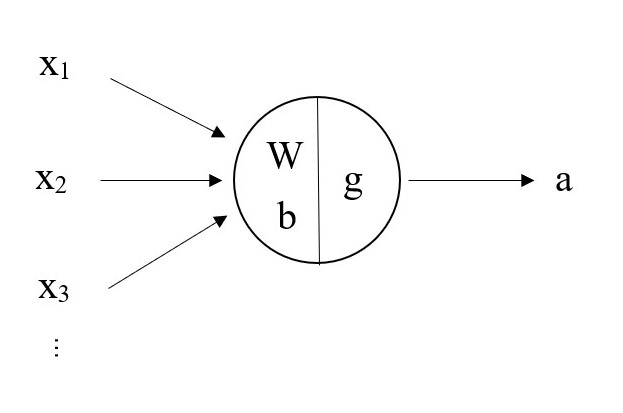
\includegraphics[width=10cm]{neuron}
    \caption{\label{fig:neuron}The model of neuron}
\end{figure}

\par The most common used activation functions are ReLU, sigmoid which are
illustrated in \autoref{fig:activation}.

\begin{figure}[H]
    \centering
    \subfigure[ReLU: $g(z) = max(0,\ z)$]{
    \begin{minipage}[t]{0.5\linewidth}
    \centering
    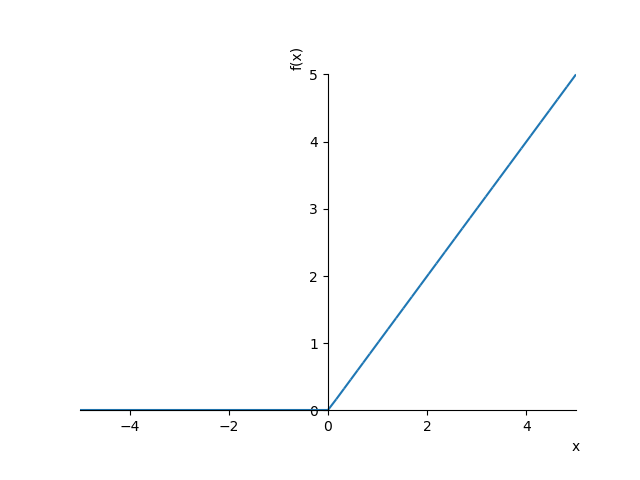
\includegraphics[width=5cm]{ReLU.png}
    \end{minipage}%
    }%
    \subfigure[sigmoid: $ \sigma(z) = \frac{1}{1+e^{(-z)}} $]{
    \begin{minipage}[t]{0.5\linewidth}
    \centering
    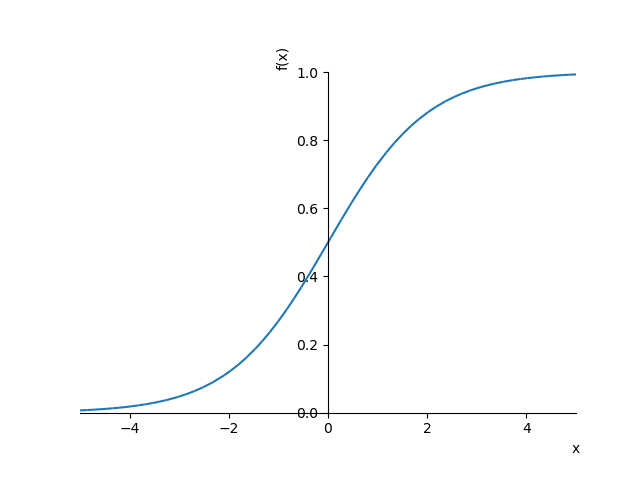
\includegraphics[width=5cm]{sigmoid.png}
    \end{minipage}%
    }%
    \centering
    \caption{\label{fig:activation}Common activation functions}
\end{figure}
\par In multi-classification tasks, softmax 
$ g(z) = \frac{e^z}{\sum\limits_{i=1}^{n}e^{z_i}},\ z \in \mathbb{R}^n\ $
is widely used in the last neuron of the neural network.

\subsection{Architecture}
Various neurons form the neural networks, and the specific formation is called
the architecture of the neural networks. Most of the architecture like 
Deep Neural Network, CNN and RNN can be regarded as a set of layers, 
each layer consists of a bunch of neurons. The output of the previous layers
serve as the input of the neurons in the current layer.

First we define the following notations: $ l $ is the index of layer,
$ L $ is the number of layers, $ n^{[l]} $ is the number of neurons 
in the $ l^{th} $ layer, $ W^{[l]} \in \mathbb{R}^{n^{[l]}\times n^{[l-1]}} $ 
and $ b^{[l]} \in \mathbb{R}^{n^{[l]}\times 1 } $ are the weights of neurons 
in the $ l^{th} $ layer, $ z^{[l]} \in \mathbb{R}^{n^{[l]}\times 1} $ is 
the caches of neurons in the $ l^{th} $ layer, 
$ a^{[l]} \in \mathbb{R}^{n^{[l]}\times 1} $ is the output of neurons 
in the $ l^{th} $ layer, 
$ g^{[l]}: \mathbb{R}^{n^{[l]}\times 1} \rightarrow \mathbb{R}^{n^{[l]}\times 1} $ 
is the activation function in the $ l^{th} $ layer.
\par The basic model of a neural network is demonstrated in \autoref{fig:shallowNN},
the input $ x $ can also be considered as the $ 0^{th} $ layer, which means
$ x = a^{[0]} $, and it is called the input layer. The last layer i.e. the $ L^{th} $
layer is called the output layer which means $ \hat{y} = a^{[L]} $. 
The remainder are called the hidden layers. 

\begin{figure}[H]
    \centering
    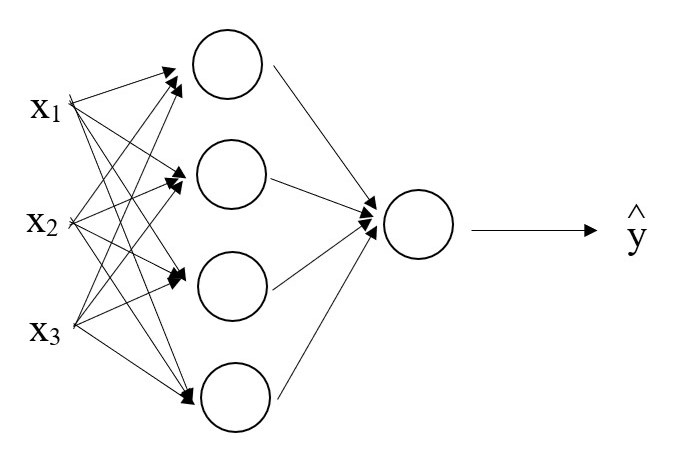
\includegraphics[width=10cm]{shallowNN}
    \caption{\label{fig:shallowNN}Shallow Neural Network}
\end{figure}

Shallow network is a simple type of neural network with only one hidden layer, 
while deep network, see \autoref{fig:deepNN}, has multiple hidden layers thus is much more complicated than
the shallow one.

\begin{figure}[H]
    \centering
    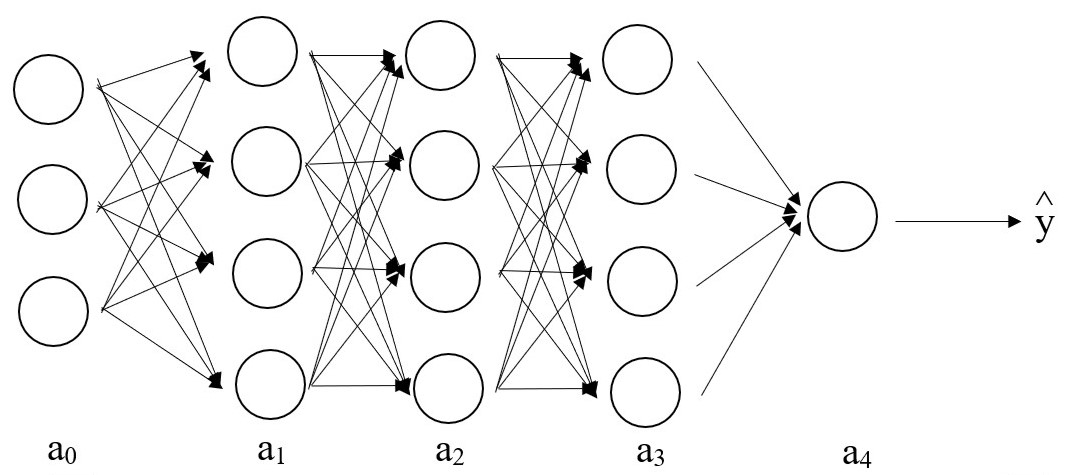
\includegraphics[width=10cm]{deepNN}
    \caption{\label{fig:deepNN}Deep Neural Network}
\end{figure}

\subsection{Loss Function}
The core of optimization problem is to minimize the cost. Given a set of labeled
data $ {x,\ y},\ x \in \mathbb{R}^{n^{[0]}\times m}, \ y \in \mathbb{R}^{1\times m} $, 
we denote that $ m $ is the number of data. We want to pick the parameters $ W,\ b $
in each neurons so that the predicted output $ \hat{y} $ is close to the true
value $ y $. To measure the difference we need to calculate the distance between
the predicted $ \hat{y}^{(i)} $ from the $ i^{th} $ sample and $ y^{(i)} $. 
For a certain distance metric $ l(\hat{y}^{(i)},\ y^{i}) $ which is also be regarded
as loss function, we can
write the total cost $ J(\hat{y},\ y) $ of the predicted $ \hat{y} $ and 
define the optimization problem as:

\begin{equation}
    \begin{split}
        & Given\ \{x,\ y\} \\
        & \mathop{\arg\min}_{W,\ b}J(\hat{y},\ y) \\
        & J(\hat{y},\ y) = \sum\limits_{i=1}^{m}l(\hat{y}^{(i)},\ y^{i})
    \end{split} 
\end{equation}

\par As for the choice of $ l $, the most widely used one is $L_2$ Norm 
i.e. Euclidean Distance $ l(x,\ y) = ||x - y||_2^2 $. Nevertheless, in
difference kinds of problems, there would be a corresponding loss function
that has the best performance. For instance, in binary classification problem,
the popular choice is binary cross-entropy: \\
$ l(x,\ y) = - x\ln(y) - (1-x)\ln(1-y) $; in multi-classification problem,
the popular choice is categorical cross-entropy: 
$ l(x,\ y) = - \sum\limits_{j=1}^{n}x^{[j]}\ln(y^{[j]}) $, where $ n $ is the 
number of classes.

\subsection{Gradient Descent}
\label{ssec:GD}
\subsubsection{Basic Intuition of GD}
Gradient descent (GD) is the foundation of a large scale of optimization algorithms
in neural networks. Imagine that you stand on the top of a mountain and
plan to go downhill, the most efficient choice is following the path that is the
steepest. Namely, the most efficient method to find the minimum of $ J $ is to
choose the gradient of $ J $ at the parameters $ W,\ b $: 
$ \nabla J(\hat{y},\ y) $ \footnote{$\nabla J(\hat{y},\ y) = 
(\frac{\partial J}{\partial W^{[1]}},\cdots,\ \frac{\partial J}{\partial W^{[L]}},\
\frac{\partial J}{\partial b^{[1]}},\cdots,\ \frac{\partial J}{\partial b^{[L]}} )^T $}
Hence, we update the parameters at the learning rate $ \alpha $:
\begin{align}
    \label{equ:GD} W^{[l]} & = W^{[l]} - \alpha\frac{\partial J}{\partial W^{[l]}} \\
    b^{[l]} & = b^{[l]} - \alpha\frac{\partial J}{\partial b^{[l]}}
\end{align}
until $ J(\hat{y},\ y) $ is small enough.

\subsubsection{Basic Convergence Analysis of GD}
It is not clear that whether GD can converge to the required global minimum
rather than local minimum. However, a notable paper by Dauphin et al. 
\parencite{dauphin2014identifying} shows that based on empirical evidence,
saddle points are bigger challenges instead of local minimum. Especially 
in high dimensional problems, saddle points are often surrounded by 
rugged plateau which dramatically slow down the speed of convergence.
More detail about the landscape of neural network will be discussed in 
\autoref{ssec:empirical}. Here we just give an basic analysis of GD algorithm.
\par Before the analysis, we need a criterion of convergence. There are mainly
two criteria: the limit point is a stationary point and the convergence of 
the function value. Apparently, the latter one is more easy to achieve.
\par In Bertsekas et al. \parencite{bertsekas1997nonlinear}, proposition 
1.2.1 to 1.2.4 give the convergence result of GD. Considering the large
scale of use of fixed learning rate, proposition 1.2.3 regarding the 
Lipschitz value is the most helpful and well-known one. And its variant
is shown in the following:
\begin{pro}
    \label{pro:ConstantConvergence}
    Let $ \{x_k\} $ be a sequence generated by GD: $ x_{k+1} = x_{k} - \alpha d_k $,
    where $ \{d_k\} $ is the gradient of $ f(x_k) $. For some $ L>0,\ 
    L \in R $  that satisfies\footnote{$ L $ is called the Lipschitz constant}:
    \begin{equation}
        ||\nabla f(x) - \nabla f(y)||\leq L||x - y||,\ \ \ \forall x,\ y \in \mathbb{R}
    \end{equation}
    If $ \forall k,\ d_k \neq 0 $ and 
    \begin{equation}
        \label{equ:learningRate}
        \epsilon \leq \alpha \leq \frac{2-\epsilon}{L}
    \end{equation}
    where $ \epsilon \in R^+ $. Then every limit point of $ \{x_k\} $ is a 
    stationary point of $f$.
\end{pro}

\begin{prf}
    Using the descent lemma\footnote{Details of descent lemma are in the 
    Appendix 1 }, we have:
    \begin{align}
        f(x_k - \alpha d_k) - f(x_k)&\leq\alpha\nabla f(x_k)^Td_k + \frac{1}{2}\alpha^2L||d_k||^2 \\
        & = \alpha ||d_k||^2(\frac{1}{2}\alpha L - 1)
    \end{align}
    The right-hand side of \autoref{equ:learningRate} yields:
    \begin{align}
        \frac{1}{2}\alpha L - 1 \leq -\frac{1}{2}\epsilon
    \end{align}
    Together with the left-hand of \autoref{equ:learningRate}:
    \begin{align}
        f(x_k) - f(x_k - \alpha d_k) \geq \frac{1}{2}\epsilon^2||d_k||^2
    \end{align}
    If $ \{x_k\} $ converge to a non-stationary point $ x $, then $ ||d_k||^2 < 0 $ 
    and $ f(x_k) - f(x_k - \alpha d_k) \rightarrow 0 $, 
    so $ ||d_k|| \rightarrow 0 $, which contradicts the assumption. Hence,
    every limit point of $ \{x_k\} $ is stationary.  \\
    \textbf{Q.E.D.}
\end{prf}

\par According to \autoref{pro:ConstantConvergence}, we can choose the 
learning rate $ \alpha = \frac{2}{L} $ and guarantee that GD will converge.
Unfortunately, for optimization in neural network, such a global Lipschitz 
constant may not exist in most cases. until now, there seems to be no obvious
way to fix the gap between the theorem and practice. In the article of Ruoyu Sun
\parencite{sun2019optimization}, a claim that may be sufficient for practitioners
is proposed: if all parameters are bounded in each iteration, with 
a small and proper learning rate $ \alpha $, GD will converge.



\subsection{Forward Propagation}
Forward propagation (FP) is a method to compute the predicted $ \hat{y} $
from the input data. To illustrate the process of FP, we use the network
shown in \autoref{fig:deepNN}. For the first layer, input of neurons is
$ A^{[0]} = (a^{[0](1)},\cdots,\ a^{[0](m)}) \in \mathbb{R}^{n^{[0]}\times m} $,
the output is $ A^{[1]} $ and the cache is $ Z^{[1]} = (z^{[1](1)},\cdots,\ z^{[1](m)}) $. 
\begin{equation}
    \begin{split}
        Z^{[1]} & = W^{[1]}A^{[0]} + b^{[1]} \\
        A^{[1]} & = g^{[1]}(Z^{[1]}) \\
        & \vdots
    \end{split}
\end{equation} 
Therefore, the general computation of the $ i^{th} $ layer is:
\begin{equation}
    \label{equ:FP}
    \begin{split}
        Z^{[l]} & = W^{[l]}A^{[l-1]} + b^{[l]} \\
        A^{[l]} & = g^{[l]}(Z^{[l]})
    \end{split}
\end{equation} 

\subsection{Backward Propagation}
Backward propagation (BP) is considered as an vital landmark in the 
development of neural networks. It highly boost the efficiency of the
computation of gradient. Different from the FP, BP starts from the output
layer of the network and goes through the network to the front. 
We denote that 
$ dA^{[l]} \triangleq \frac{\partial J}{\partial A^{[l]}} 
\in \mathbb{R}^{n^{[l]}\times m} $,
$ dZ^{[l]} \triangleq \frac{\partial J}{\partial Z^{[l]}} 
\in \mathbb{R}^{n^{[l]}\times m} $,
$ dW^{[l]} \triangleq \frac{\partial J}{\partial W^{[l]}} 
\in \mathbb{R}^{n^{[l]}\times n^{[l-1]}} $ and
$ db^{[l]} \triangleq \frac{\partial J}{\partial b^{[l]}} 
\in \mathbb{R}^{n^{[l]}\times 1} $.
For the $ L^{th} $ layer, we can calculate the gradient by the following
way\footnote{the operator $*$ is element-wise multiplication}
\footnote{the update of parameters in GD involve the complete data set, 
while in the variant of GD like SGD and mini-batch GD, only part of the data
contribute to the update process in each iteration}:
\begin{equation}
    \begin{split}
        dA^{[L]} & = \frac{\partial J}{\partial A^{[L]}} \\
        dZ^{[L]} & = dA^{[L]}*g^{[L]'}(Z^{[L]}) \\
        dW^{[L]} & = \frac{1}{m}dZ^{[L]}A^{[L-1]T} \\
        db^{[L]} & = \frac{1}{m}dZ^{[L]} \\
        dA^{[L-1]} & = W^{[L-1]T}dZ^{[L]} \\
        dZ^{[L-1]} & = dA^{[L-1]}*g^{[L-1]'}(Z^{[L-1]}) \\
        & \vdots
    \end{split}
\end{equation}
Suppose the loss function of the output layer is binary cross-entropy: \\
$ l(a^{[L]},\ y) = - y\ln(a^{[L]}) - (1-y)\ln(1-a^{[L]}) $, then 
the BP process can be written as:
\begin{equation}
    \label{equ:BP}
    \begin{split}
        dZ^{[L]} & = A^{[L]} - y \\
        dW^{[L]} & = \frac{1}{m}dZ^{[L]}A^{[L-1]T} \\
        db^{[L]} & = \frac{1}{m}dZ^{[L]} \\
        & \vdots \\
        dA^{[l]} & = W^{[l]T}dZ^{[l+1]} \\
        dZ^{[l]} & = (W^{[l]T}dZ^{[l+1]})*g^{[l]'}(Z^{[l]}) \\
        dW^{[l]} & = \frac{1}{m}dZ^{[l]}A^{[l-1]T} \\
        db^{[l]} & = \frac{1}{m}dZ^{[l]}
    \end{split}
\end{equation}